\documentclass{beamer}
\usepackage[absolute,overlay]{textpos}
\usepackage{pifont}
\setbeamertemplate{bibliography item}[text]
\setbeamertemplate{navigation symbols}{}
\setbeamertemplate{caption}[numbered] 
\setbeamerfont{caption}{size=\scriptsize}
\setbeamertemplate{footline}[frame number]

\setbeamerfont{page number in head/foot}{size=\large}
\setbeamertemplate{footline}[frame number]

\usepackage{units}
\usepackage{amssymb}
\usepackage{color}
\definecolor{offyellow}{cmyk}{0, 0, 1, .2}
\usepackage{movie15}

\newcommand\FrameText[1]{
\begin{textblock}{16}(1,2.5)
\raggedright #1
\end{textblock}}

\begin{document}

\addtobeamertemplate{frametitle}{}{
\begin{textblock}{16}(0,0)

\includegraphics[scale=0.5]{Header.png}
\end{textblock}}

\begin{frame}
\frametitle{1}
\begin{picture}(0.0,0.0)
\put(-28.45,-142){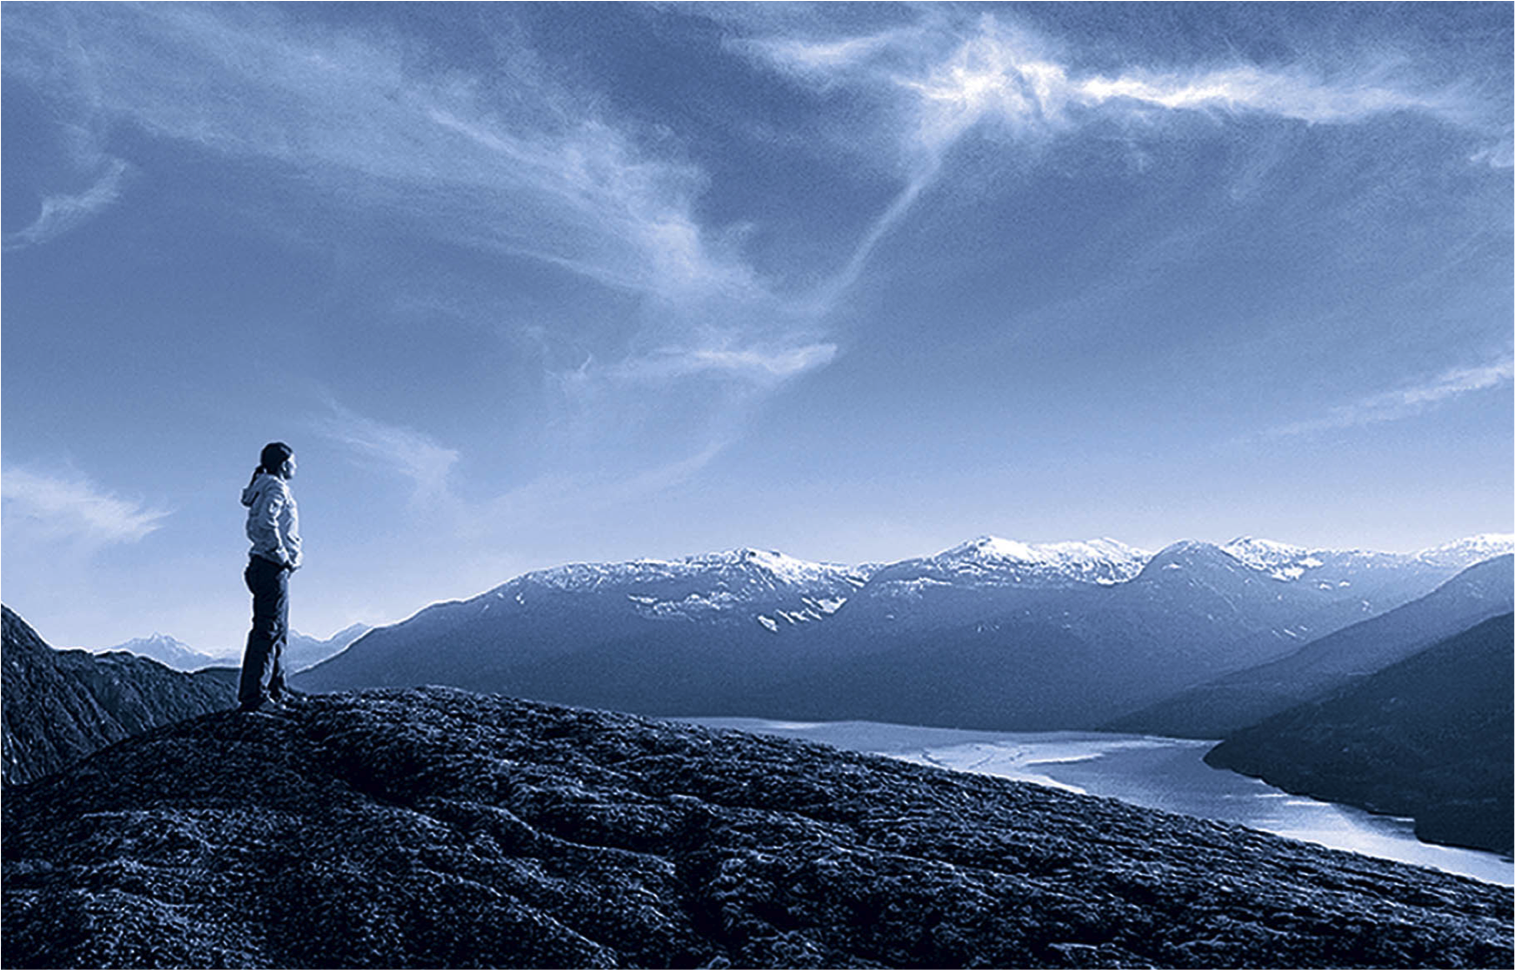
\includegraphics[width=\paperwidth]{FrontPage.png}}
\end{picture}
\FrameText{
\textcolor{white}{\bf{\LARGE The Effects of two Parameters on idealised Convecitve Boundary Layer Entrainment}}\\
\textcolor{white}{\bf{\LARGE MSc Defense}}\\
\textcolor{white}{\bf{Niamh Chaparro}}}
\end{frame}

\begin{frame}
\frametitle{2}
%\FrameText{what is the convective boundary layer and its entrainment zone}
\begin{figure}
\centering
\includegraphics[scale = 1, trim = 0 15 0 0, clip]{/newtera/tera/phil/nchaparr/tera2_cp/nchaparr/ubcdiss/pngs/cbl}
\fontsize{12pt}{7.2}\selectfont
\caption{Representation of the time evolution of the convective boundary layer adapted from Stull 1988.}
\end{figure}
\end{frame}


\begin{frame}
\frametitle{3}
\fontsize{12pt}{7.2}\selectfont
\FrameText{Knowledge of the convective boundary layer (CBL)\\
 and its entrainment zone (EZ) is important because:
 \vspace{10mm}
\begin{itemize}
\item CBL height is needed to calculate CBL concentrations
\vspace{10mm}
\item knowledge of EZ depth and lifting condensation level\\
 enables cloud cover prediction
\vspace{10mm}
\item parametrizations for both are required in\\ 
global circulation models (GCMs)
\end{itemize}
%\textcolor{white}{\bf{\LARGE }}\\
%\textcolor{white}{\bf{\LARGE }}\\
%\textcolor{white}{\bf{, MSc , }}
}
\end{frame}

\begin{frame}
\frametitle{4}
\fontsize{12pt}{7.2}\selectfont
\FrameText{Three types of CBL entrainment Studies:
\vspace{10mm}
\begin{itemize}
\item measurement based
\vspace{10mm} 
\item numerical models that use the Navier Stokes Equations: large eddy simulation (LES), direct numerical simulation (DNS)
\vspace{10mm}
\item bulk models based on average quantities and simplified profiles
\end{itemize}
}

\end{frame}
\begin{frame}
\frametitle{4}
\fontsize{12pt}{7.2}\selectfont
\FrameText{There is ongoing discussion about:
\vspace{10mm}
\begin{itemize}
\item the critical resolution for capturing entrainment
\vspace{10mm}
\item the multitude of definitions (e.h. CBL height, EZ boundaries)
\vspace{10mm}
\item the form of the relationships of CBL growth\\ 
($w_{e}$ entrainment rate) and EZ depth ($\Delta h$)  to \\
convecitive Richardson number ($Ri$ defined later)
\end{itemize}
}
\end{frame}


\begin{frame}
\frametitle{4}
\fontsize{12pt}{7.2}\selectfont
\FrameText{I set out to:
\vspace{10mm}
\begin{itemize}
\item apply resolution at which convergence occured\\
(Peter P. Sullivan and Edward G. Patton 2011)
\vspace{10mm}  
\item define CBL height and EZ limits based on the average \\
$\theta$ profile
\vspace{10mm}
\item investigate the resulting relationships of $w_{e}$ and \\
 $\Delta h$ to $Ri$:
\end{itemize}
}
\end{frame}


\begin{frame}
\frametitle{5}
\fontsize{12pt}{7.2}\selectfont
\FrameText{I modeled a dry idealized CBL, wihout large scale winds\\using the LES System for Atmospheric Modelling (SAM):
\vspace{10mm}
\begin{itemize}
\item Anelastic equations of motion
\vspace{10mm} 
\item Liquid/Ice static energy ($h_{l}$) is the prognosed thermodynamical variable
\vspace{10mm}
\item First order Smagorinksi closure
\vspace{10mm}
\item Fully stagered Arakawa c grid
\vspace{10mm}
\item three dimensional positive definite advection of scalars
\end{itemize}
}
\end{frame}

\begin{frame}
\frametitle{6}
\begin{table}[!ht]
\fontsize{12pt}{7.2}\selectfont
\caption{Table of 10-ensemble Runs in terms of the two external parameters: surface heat flux ($\overline{w^{'} \theta^{'}_{s}}$) and initial lapse rate $\gamma$}
    \centering
    \begin{tabular}{ | l | l | l | l |}
    \hline
    $\overline{w^{'}\theta^{'}_{s}}$ / $\gamma$ & 10 (K/Km) & 5 (K/Km) & 2.5 (K/Km) \\ \hline
     150 (W/m2)& \hspace{1.95mm} {\color{red} \ding{116}} 150/10 &\hspace{3.45mm}{\color{red} \ding{108}} 150/5\footnotemark &  \\ \hline
     100 (W/m2)& \hspace{2mm} {\color{black} \ding{116}} 100/10 & \hspace{2mm} {\color{black} \ding{108}} 100/5 & \\ \hline
     60 (W/m2) & \hspace{2mm} {\color{offyellow} \ding{116}} 60/10 & \hspace{2mm} {\color{offyellow} \ding{108}} 60/5 & \hspace{2mm} {\color{offyellow} \ding{72}} 60/2.5\\ \hline
\end{tabular}
\label{fig:tableofruns}   
\end{table}
\footnotetext{Incomplete run: EZ exceeded high resolution vertical grid after 7 hours}
\end{frame}

\begin{frame}
\frametitle{3}
\begin{figure}[htbp]
    \centering
    %plot_height.py[master 1573b9d] h vs time plot
    \includegraphics[scale=.45]{/newtera/tera/phil/nchaparr/python/Plotting/Dec252013/pngs/height_defs.pdf}
\fontsize{12pt}{7.2}\selectfont
    \caption[]{Height definitions based on the average vertical profiles.\\
$\theta_{0}$ is the initial potential temperature.}
    \label{fig:hdefs}   % label should change
\end{figure}
\end{frame}

\begin{frame}
\frametitle{7}
\begin{table}[htbp]
\caption[]{Definitions based on the vertical $\overline{\theta}$ profile in Figure 2.}
    \begin{center}
%\centerline{
    \begin{tabular}{ p{1cm} p{2cm} p{2cm}  p{2cm}  p{2cm} p{2.5cm} }
    %\hline
      CBL& ML $\overline{\theta}$ & Deardorff & $\theta$ Jump &Richardson\\
      Height&($\overline{\theta}_{ML}$)&Velocity&($\Delta \theta$)&Number\\
            &&Scale ($w^{*}$)&&($Ri$) \\ \hline 
       $h$  &$\frac{1}{h}\int^{h}_{0}\overline{\theta}(z)dz$ & $\left( \frac{gh}{\overline{\theta}}(\overline{w^{'}\theta^{'}})_{s} \right)^{\frac{1}{3}}$& $\overline{\theta}(h_{1})-\overline{\theta}(h_{0})$ & $\frac{\frac{g}{\overline{\theta}_{ML}}\Delta \theta h}{w^{*2}}$  \\ [.3cm] \hline
      \end{tabular}
%}
\label{tab:reldefs}   
\end{center}    
\end{table}
\end{frame}

\begin{frame}
\frametitle{7}
%\begin{frame}[t]{}
 \begin{figure}[ht]
   \includemovie[autoplay, repeat=50]{8cm}{6cm}{theta.avi}
 \end{figure}
%\end{frame}
%\FrameText{\bf{\large}}
\end{frame}

\begin{frame}
\frametitle{8}
\fontsize{12pt}{7.2}\selectfont
\begin{figure}
\centering
\includegraphics[scale=.4]{/newtera/tera/phil/nchaparr/python/Plotting/Mar52014/pngs/rss_fit_high}
\caption{Local $\theta$ profile at a single horizontal point where\\ 
height is relatively high, at 5 simulated hours (left).\\
On the right Tri-linear fit to the local $\theta$ profile with \\
a line for each of the 3 layers: mixed layer (ML), EZ and free \\
atmosphere (FA).}
\end{figure}
\end{frame}

\begin{frame}
\frametitle{9}

\begin{figure}
\fontsize{12pt}{7.2}\selectfont
\centering
\includegraphics[scale = .4]{/newtera/tera/phil/nchaparr/python/Plotting/Mar52014/pngs/rss_fit_low}
\caption{As in previous slide but at a point where height is relatively low.}
\end{figure}
\end{frame}

\begin{frame}
\frametitle{10}
\fontsize{12pt}{7.2}\selectfont
%\FrameText{Now look at local CBL height distributions}
\begin{figure}
\begin{columns}[T]
   \begin{column}{.5\textwidth}
   \centering
   \includegraphics[scale = 0.28]{/newtera/tera/phil/nchaparr/python/Plotting/Dec252013/pngs/ML_Height_hist_10} 
   \end{column} 
   
   \begin{column}{.5\textwidth}
    \centering
    \includegraphics[scale = 0.28]{/newtera/tera/phil/nchaparr/python/Plotting/Dec252013/pngs/Scaled_ML_Height_hist_10}
   \end{column}     
\end{columns}
\caption{Distribution of local ML heights (left).\\
PDF of local ML heights scaled by $h$ (right).\\
$h$ is the CBL height based on maximum average\\
 vertical $\theta$ gradient.}
\end{figure}
\end{frame}

\begin{frame}
\frametitle{11}
\fontsize{12pt}{7.2}\selectfont
%\FrameText{Now look at local (CBL) height distributions
\begin{figure}
\begin{columns}[T]
   \begin{column}{.5\textwidth}
   \includegraphics[scale = 0.28]{/newtera/tera/phil/nchaparr/python/Plotting/Dec252013/pngs/ML_Height_hist_5} 
   \end{column} 
   
   \begin{column}{.5\textwidth}
    \includegraphics[scale = 0.28]{/newtera/tera/phil/nchaparr/python/Plotting/Dec252013/pngs/Scaled_ML_Height_hist_5}
   \end{column}     
\end{columns}
\caption{As previous slide but with lower $\gamma$}
\end{figure}
\end{frame}

\begin{frame}
\frametitle{12}
\fontsize{12pt}{7.2}\selectfont
%\FrameText{Now look at local (CBL) height distributions
\begin{figure}
\begin{columns}[T]
   \begin{column}{.5\textwidth}
   \includegraphics[scale = 0.28]{/newtera/tera/phil/nchaparr/python/Plotting/Dec252013/pngs/ML_Height_hist_2point5} 
   \end{column} 
   
   \begin{column}{.5\textwidth}
    \includegraphics[scale = 0.28]{/newtera/tera/phil/nchaparr/python/Plotting/Dec252013/pngs/Scaled_ML_Height_hist_2point5}
   \end{column}     
\end{columns}
\caption{As previous slide but with lower $\gamma$}
\end{figure}
\end{frame}


\begin{frame}
\frametitle{13}
\FrameText{\bf{\large Conclusion:}
\vspace{5mm}
\begin{itemize}
\item \bf{\large The scaled lowest local CBL heights decrease\\
with decreased stability}
\end{itemize}
}
\end{frame}

\begin{frame}
\frametitle{14}
%\FrameText{Now look at EZ based on the Average profile:
%}
\fontsize{12pt}{7.2}\selectfont
\begin{figure}
\centering
\includegraphics[scale=.4]{/newtera/tera/phil/nchaparr/python/Plotting/Nov302013/pngs/theta_flux_profs}
\caption{Evolution of (left) Ensemble and horizontally averaged $\theta$,\\
(middle) its vertical gradient ($\frac{\partial \overline{\theta}}{\partial z}$)\\
and (right) vertical heat flux ($\overline{w^{'}\theta^{'}}$)}
\end{figure}
\end{frame}

\begin{frame}
\frametitle{15}
%\FrameText{Now look at EZ based on the Average profile:
%}
\fontsize{12pt}{7.2}\selectfont
\begin{figure}
\centering
\includegraphics[scale=.4]{/newtera/tera/phil/nchaparr/python/Plotting/Dec252013/pngs/theta_grad_profs}
\end{figure}
\end{frame}

\begin{frame}
\frametitle{16}
\FrameText{Now look at EZ based on the Average profile:
}
\begin{figure}
\centering
\includegraphics[scale=.4]{/newtera/tera/phil/nchaparr/python/Plotting/Dec252013/pngs/scaleddeltahstime}
\end{figure}

\end{frame}

\begin{frame}
\frametitle{17}
\FrameText{\bf{\large Conclusion:}
\begin{itemize}
\item \textcolor{gray}{The scaled lowest local heights decrease with decreased stability}
\item \bf{\large scaled lower EZ boundary increases with increased $Ri$}\\
\end{itemize}
}
\end{frame}

\begin{frame}
\frametitle{18}
\FrameText{Now look at relationship of scaled EZ depth to Richardson number:
}
\begin{figure}
\centering
\includegraphics[scale=.4]{/newtera/tera/phil/nchaparr/python/Plotting/Dec252013/pngs/scaleddeltahinvri}
\end{figure}

\end{frame}

\begin{frame}
\frametitle{19}
\FrameText{Now look at relationship of scaled EZ depth to Richardson number $\frac{\Delta h}{h} \propto Ri ^{b}$:
}
\begin{figure}
\centering
\includegraphics[scale=.4]{/newtera/tera/phil/nchaparr/python/Plotting/Dec252013/pngs/scaleddeltahinvri}
\end{figure}

\end{frame}

\begin{frame}
\frametitle{20}
\FrameText{\bf{\large Conclusion}:
\begin{itemize}
\item \textcolor{gray}{scaled lowest local heights increase with increased stability}
\item \textcolor{gray}{scaled lower boundary based on average profile increases with increased $Ri$} \\
\item \bf{ \large curves representing  $\frac{\Delta h}{h} \propto Ri ^{b}$}\\
\bf{ \large group according to $\gamma$ when EZ is defined based on $\frac{\partial \overline{\theta}}{\partial z}$}
\end{itemize}
}
\end{frame}

\begin{frame}
\frametitle{21}
\FrameText{But if I define the EZ based on $\frac{\frac{\partial \overline{\theta}}{\partial z}}{\gamma}$ 
}

\begin{columns}[T]
   \begin{column}{.5\textwidth}
   \includegraphics[scale = 0.28]{/newtera/tera/phil/nchaparr/python/Plotting/Dec252013/pngs/theta_grad_profs} 
   \end{column} 
   
   \begin{column}{.5\textwidth}
    \includegraphics[scale = 0.28]{/newtera/tera/phil/nchaparr/python/Plotting/Dec252013/pngs/scaled_theta_grad_profs}
   \end{column}     
\end{columns}
\end{frame}

\begin{frame}
\frametitle{22}
\FrameText{The order of lower boundary heights is reversed -- increased $\gamma$ yields higher lower EZ boundary 
}

\begin{columns}[T]
   \begin{column}{.5\textwidth}
   \includegraphics[scale = 0.28]{/newtera/tera/phil/nchaparr/python/Plotting/Dec252013/pngs/theta_grad_profs_zoomin} 
   \end{column} 
   
   \begin{column}{.5\textwidth}
    \includegraphics[scale = 0.28]{/newtera/tera/phil/nchaparr/python/Plotting/Dec252013/pngs/scaled_theta_grad_profs_zoomin}
   \end{column}     
\end{columns}
\end{frame}

\begin{frame}
\frametitle{23}
\FrameText{:
}
\begin{figure}
\centering
\includegraphics[scale=.4]{/newtera/tera/phil/nchaparr/python/Plotting/Dec252013/pngs/scaleddeltahinvri_4}
\end{figure}

\end{frame}

\begin{frame}
\frametitle{24}
\FrameText{\bf{\large Conclusion}:
\begin{itemize}
\item \textcolor{gray}{scaled lowest local heights increase with increased stability}
\item \textcolor{gray}{scaled lower boundary based on average profile increases with increased stability and over time}
\item \bf{\large curves representing  $\frac{\Delta h}{h} \propto Ri ^{b}$ group according to $\gamma$ when EZ is defined based on $\frac{\partial \overline{\theta}}{\partial z}$ but collapse when EZ is based on $\frac{\frac{\partial \overline{\theta}}{\partial z}}{\gamma}$} 
\end{itemize}
}
\end{frame}

\begin{frame}
\frametitle{25}
\FrameText{The downward moving warm potential temperature fluctuations ($\theta^{'+}_{h} \ where w^{'}<0$) at $h$ ``warms'' the air below
}
\end{frame}

\begin{frame}
\frametitle{26}
\FrameText{$\theta^{'+}_{h} \ where w^{'}<0$ is effectively scaled by $\delta h \gamma$, where $\delta h = h_{1} - h$:
}
\begin{columns}[T]
   \begin{column}{.5\textwidth}
   \includegraphics[scale = 0.28]{/newtera/tera/phil/nchaparr/python/Plotting/Dec252013/pngs/downwarm_theta.pdf} 
   \end{column} 
   
   \begin{column}{.5\textwidth}
    \includegraphics[scale = 0.28]{/newtera/tera/phil/nchaparr/python/Plotting/Dec252013/pngs/scaled_downwarm_theta2.pdf}
   \end{column}     
\end{columns}
\end{frame}

\begin{frame}
\frametitle{27}
\FrameText{Why $\delta h \gamma$ is so effective:}
\begin{figure}
\includegraphics[scale=.4]{/newtera/tera/phil/nchaparr/tera2_cp/nchaparr/ubcdiss/pngs/deltagamma}
\end{figure}
\end{frame}

\begin{frame}
\frametitle{28}
\FrameText{\bf{\large Conclusion:}
\begin{itemize}
\item \textcolor{gray}{scaled lowest local heights increase with increased stability}
\item \textcolor{gray}{scaled lower boundary based on average profile increases with increased $Ri$}
\item \textcolor{gray}{curves representing  $\frac{\Delta h}{h} \propto Ri ^{b}$ group according to $\gamma$ when EZ is defined based on $\frac{\partial \overline{\theta}}{\partial z}$ but collapse when EZ is based on $\frac{\frac{\partial \overline{\theta}}{\partial z}}{\gamma}$} 
\item \bf{\large downward moving positive potential temperature fluctuations at $h$ are scaled by $\delta h \gamma$}
\end{itemize}
}
\end{frame}

\begin{frame}
\frametitle{29}
\FrameText{The exponent of $\frac{\Delta h}{h} \propto Ri^{b}$ is in line with theory and results of other studies, and changes:
}
\begin{figure}
\centering
\includegraphics[scale=.4]{/newtera/tera/phil/nchaparr/python/Plotting/Dec252013/pngs/loglog_scaleddeltahinvri_4}
\end{figure}
\end{frame}

\begin{frame}
\frametitle{30}
\FrameText{As does the exponent of $\frac{w_{e}}{w^{*}} \propto  Ri^{a}$:}
\begin{figure}
\includegraphics[scale=.4]{/newtera/tera/phil/nchaparr/python/Plotting/Dec252013/pngs/scaledweinvri_Delta}
\end{figure}
\end{frame}

\begin{frame}
\frametitle{31}
\FrameText{\bf{\large Conclusion:}
\begin{itemize}
\item \bf{\large scaled lowest local heights increase with increased stability}
\item \bf{\large scaled lower boundary based on average profile increases with increased $Ri$}
\item \bf{\large curves representing  $\frac{\Delta h}{h} \propto Ri ^{b}$ group according to $\gamma$ when EZ is defined based on $\frac{\partial \overline{\theta}}{\partial z}$ but collapse when EZ is based on $\frac{\frac{\partial \overline{\theta}}{\partial z}}{\gamma}$} 
\item \bf{\large downward moving positive potential temperature fluctuations at $h$ are scaled by $\delta h \gamma$}
\item \bf{\large there is a change in entrainment regime with increased richardson number}
\end{itemize}
}
\end{frame}

\begin{frame}
\frametitle{32}
\FrameText{\bf{\large Conclusion:}
\begin{itemize}
\item \bf{\large scaled EZ depth decreases with increasd Richardson number}
\item \bf{\large $\frac{\partial \overline{\theta}}{\partial z}$ in the upper (CBL) and the downward moving positive potential temperature fluctuations at $h$ are depend on $\gamma$}
\item \bf{\large there is a change in entrainment regime with increased richardson number}
\end{itemize}
}
\end{frame}

\begin{frame}
\frametitle{2}
\FrameText{\bf{\large References}}
\begin{thebibliography}{99}
\bibitem{SullPat} Peter P. Sullivan and Edward G. Patton 2011: \emph{The Effect of Mesh Resolution on Convective Boundary Layer Statistics and Structures Generated by Large Eddie Simulation}. Journal of the Atmospheric Sciences, 58, 2395-2415.
\bibitem{Stull-BLMetIntro} Roland Stull 1988: \emph{An Introduction to Boundary Layer Meteorology}. Kluwer Academic Publishers.

\end{thebibliography}
\end{frame}


\end{document}


